\documentclass[11pt,reqno]{amsart}
\usepackage[T1]{fontenc}
\usepackage[utf8]{inputenc}
\usepackage{amsmath,amssymb,amsthm}
\usepackage[letterpaper,margin=0.75in]{geometry}
\usepackage{graphicx}
\graphicspath{{../images/}}
\usepackage{booktabs}
\usepackage{algorithm}
\usepackage{algpseudocode}
\usepackage[hidelinks]{hyperref}
\DeclareMathOperator{\vol}{vol}
\DeclareMathOperator{\conv}{conv}
%% Artifact references: a second reference group pointing into the repository
%% rather than the literature, numbered [R1], [R2], ... so that it cannot be
%% confused with the bibliography. Set \repobase and \repocommit once; every
%% link and every citation follows.
\newcommand{\repobase}{https://github.com/csabamedgyeswork/inscribed-polytopes}
\newcommand{\repocommit}{main}
\newcommand{\repohref}{\href{\repobase}{\texttt{\repobase}}}
% \nolinkurl rather than \texttt so a long path may break after a slash.
\newcommand{\artpath}[1]{\href{\repobase/tree/\repocommit/#1}{\nolinkurl{#1}}}
\newcounter{artifact}
\newenvironment{artifactlist}
{\sloppy % entries are mostly path, so prefer stretched spaces to overrun
\begin{list}{[R\arabic{artifact}]}
{\usecounter{artifact}%
\setlength{\labelwidth}{3.1em}\setlength{\leftmargin}{3.7em}%
\setlength{\labelsep}{0.6em}\setlength{\itemsep}{0.15ex}%
\setlength{\parsep}{0pt}}}
{\end{list}}
\newcommand{\artifact}[3]{\item\label{art:#1}\artpath{#2}, #3}
\newcommand{\artref}[1]{\hyperref[art:#1]{[R\ref*{art:#1}]}}
\newtheorem{theorem}{Theorem}[section]
\newtheorem{lemma}[theorem]{Lemma}
\theoremstyle{definition}
\newtheorem{definition}[theorem]{Definition}
\title[Maximum-volume inscribed polytopes]
{Maximum-volume polytopes inscribed in the unit sphere:
a computational reproduction of known results}
\author{Csaba Medgyes}
\email{csaba.medgyes.work@gmail.com}
\begin{document}
\begin{abstract}
This work presents an experimental methodology for the study of
maximum-volume polytopes with $n$ vertices inscribed in the unit sphere.
Rather than introducing new mathematical results, we use the proposed
approach to reproduce and verify a collection of existing ones. Working from
the signed-volume polynomial and the Berman--Hanes local optimality condition, a
single implementation sweeps every combinatorial type of simplicial polytope
and reproduces the published record on $\mathbb{S}^{2}$ for
$4 \leq n \leq 12$ and on $\mathbb{S}^{3}$ for $n \leq 8$, with every number
labelled by an evidence level derived from its own data. We also note a
failure mode affecting relaxation-based approaches: the signed-volume
polynomial attains spurious maxima at self-intersecting configurations
satisfying the optimality condition exactly. In four dimensions the sweep
winners for $6 \leq n \leq 8$ are convex hulls of two regular polygons in
orthogonal planes.
\end{abstract}
\maketitle
\section{Introduction}
\label{sec:intro}

Among the convex polytopes with $n$ vertices inscribed in the unit sphere
$\mathbb{S}^{d-1}$, which has the largest volume? Fejes T\'{o}th posed the
three-dimensional case in \emph{Regular Figures}, where an inequality already
settles $n = 4, 6, 12$ as the regular tetrahedron, octahedron and icosahedron
\cite[p.~263]{fejes-toth-1964}, as restated in \cite{horvath-2016-survey}. The
remaining cases have resisted a uniform treatment, and progress has come case
by case.

In three dimensions the line runs as follows. Goldberg stated a conjecture on
the shape of the extremal polyhedron for the dual isoperimetric problem
\cite{goldberg-1935}; Grace transferred the question to the inscribed setting
and ran an early computer search \cite{grace-1963}; Bowen and Fisk supplied the
isomorph-free enumeration of sphere triangulations that made case analysis
possible \cite{bowen-fisk-1967}. Berman and Hanes then introduced the local
optimality condition now called Property Z, proved that a maximiser is
simplicial, and settled $n = 5, 7, 8$ \cite{berman-hanes-1970}. The next case
took fifty-six years: Hoehner and Ledford resolved $n = 9$, the maximiser being
a triaugmented triangular prism of volume $3\sqrt{2\sqrt{3}-3}$
\cite{hoehner-ledford-2026}. Beyond this the record is numerical. Mutoh
reported a computer search for $4 \leq n \leq 30$ \cite{mutoh-2003}, and
Hardin, Sloane and Smith tabulate putatively optimal configurations for
$4 \leq n \leq 130$ \cite{hardin-sloane-smith}; the values at $n = 10$ and
$n = 11$ are recorded as conjectures in \cite{oeis-a339262,oeis-a339263}. No
optimality proof is known for $n = 10$, $n = 11$ or any $n \geq 13$.

In higher dimensions Horv\'{a}th and L\'{a}ngi extended Property Z and
simpliciality to every dimension and solved $n = d+2$ outright, $n = d+3$ for
odd $d$, and $n = d+3$ for even $d$ among noncyclic polytopes; they also showed
that the maximal-volume inscribed cross-polytope is the regular one
\cite{horvath-langi-2016}. Exhaustive work in four dimensions additionally
needs to know which combinatorial types admit an inscribed realisation at all,
the problem Steiner raised in 1832 \cite{steiner-1832}. Hodgson, Rivin and
Smith characterised it in three dimensions
\cite{hodgson-rivin-smith-1992,dillencourt-smith-1996}, but no comparable
characterisation is known in higher dimensions \cite{padrol-ziegler-2016};
Firsching's inscribed rational realisations supply the answer for $d = 4$,
completely for $n \leq 8$ \cite{firsching-2017}.

This work presents an experimental methodology rather than new mathematics. A
single implementation, applied uniformly instead of case by case, reproduces
and verifies results spread across these papers, and every number it reports is
labelled with the strength of the evidence behind it. Claims about our own
computations and code carry a second kind of reference, written [R$k$] and
listed under \emph{Code and data} \artref{reproduce}. In summary:

\begin{enumerate}
  \item The published record is reproduced on $\mathbb{S}^{2}$ for
    $4 \leq n \leq 12$ and on $\mathbb{S}^{3}$ for
    $n \leq 8$ (Sections~\ref{sec:results3} and \ref{sec:results4}). At $d = 4$,
    $n = 7, 8$ the sweep ranges over every combinatorial type, where the
    published optimality results are restricted to a class, so it covers a
    wider class of polytopes, though only numerically.
  \item Every case carries an evidence level recomputed from its own per-type
    data rather than asserted in prose, so a claim cannot drift ahead of the
    numbers supporting it (Section~\ref{sec:method}).
  \item We note a failure mode affecting relaxation-based approaches. The
    signed-volume polynomial attains spurious maxima at self-intersecting
    configurations which satisfy Property Z exactly, and ascent converges to
    them from a large share of starts; on such a type every valid bound on the
    bare polynomial lies above the true maximum and so excludes nothing
    (Section~\ref{sec:trap}). The inequality that survives still supports a
    triage of combinatorial types.
  \item In four dimensions the sweep winners for $6 \leq n \leq 8$ are convex
    hulls of two regular polygons in orthogonal planes, so their volumes share
    one closed form (Section~\ref{sec:results4}).
\end{enumerate}

Nothing reported here is a certified bound, and the distinction between what is
computed and what is proved is recorded throughout.

\section{Preliminaries}
\label{sec:preliminaries}

\subsection{Notation}

We follow the notation of Horv\'{a}th and L\'{a}ngi
\cite[Sections~1--2]{horvath-langi-2016}. The unit sphere of $\mathbb{R}^{d}$
is $\mathbb{S}^{d-1}$, $o$ is the origin, $V(P)$ is the vertex set of a
polytope $P$, and $\mathcal{P}_{d}(n)$ is the family of $d$-dimensional
polytopes with $n$ vertices inscribed in $\mathbb{S}^{d-1}$. For
$P \in \mathcal{P}_{d}(n)$, $\mathcal{C}(P)$ is a simplicial complex with
$|\mathcal{C}(P)| = \operatorname{bd} P$ whose vertices are exactly the points
of $V(P)$, with each of its $(d-1)$-simplices $(p_{i_{1}},\dots,p_{i_{d}})$
oriented outward; these simplices are the
\emph{facets} of $\mathcal{C}(P)$.

\subsection{The signed-volume identity}

A combinatorial type is recorded as an oriented simplicial $(d-1)$-sphere
$\mathcal{C}$ with facet set $\mathcal{F}$, each facet an ordered $d$-tuple of
vertex indices. For a configuration $p = (p_{1},\dots,p_{n}) \in
(\mathbb{S}^{d-1})^{n}$ put
\begin{equation}
  \label{eq:signed-volume}
  D(p) \;=\; \sum_{F \in \mathcal{F}} \det\bigl(p_{F_{0}},\dots,p_{F_{d-1}}\bigr).
\end{equation}
If $p$ realises $\mathcal{C}$ as a convex polytope $P$ with its facets oriented
outward, then $d!\,\vol_{d}(P) = D(p)$; for $d = 3$ this is
\cite[Lemma~3.5]{hoehner-ledford-2026}, which holds even if $o \notin P$
\cite[Remark~3.6]{hoehner-ledford-2026}, and the same argument works in every
dimension. A maximiser contains $o$ in its interior
\cite[Lemma~3.3]{hoehner-ledford-2026}, but our method does not use this:
intermediate configurations need not contain $o$, so we orient each facet
against the centroid of the vertices.
Rotating or reflecting all the points leaves the volume unchanged, so a
maximiser is only unique up to rotation and reflection, and the symmetry groups
we report are the rotations and reflections that map its points onto
themselves.

We emphasise that $D$ is defined on all of $(\mathbb{S}^{d-1})^{n}$, where it
need not compute a polytope volume. The consequences of this are the subject of
Section~\ref{sec:trap}.

\subsection{How the volume depends on one vertex}

Each summand of \eqref{eq:signed-volume} is, up to the factor $d!$, a cone
with apex $o$ over one facet. Moving a single vertex $p_{i}$ changes only the
cones over facets that contain it. In such a cone, the other $d-1$ vertices of
the facet together with $o$ form a fixed base and $p_{i}$ is the remaining
corner, so its volume is the base area times the height of $p_{i}$ above the
base, divided by $d$: a linear function of $p_{i}$. Adding these up,
\begin{equation}
  \label{eq:multilinear}
  D(p) \;=\; \langle n_{i}, p_{i}\rangle + c_{i},
  \qquad
  n_{i} \;=\; \sum_{F \ni i} p_{j_{1}^{F}} \times \cdots \times p_{j_{d-1}^{F}},
\end{equation}
where $c_{i}$ collects the facets that miss $i$, and each term of $n_{i}$ is the
cross product of the other vertices of $F$ after reordering $F$ so that $i$
comes first, with the sign flipped if that takes an odd number of swaps. For $d = 3$ this is the ordinary cross product of two
vectors; in general $v_{1} \times \cdots \times v_{d-1}$ is the vector
perpendicular to $v_{1},\dots,v_{d-1}$ whose length is the volume of the
parallelotope they span, with $\langle x, v_{1} \times \cdots \times
v_{d-1}\rangle = \det(x, v_{1},\dots,v_{d-1})$. So $n_{i}$ adds up one vector
per facet at $i$, each perpendicular to the fixed base of its cone and as long
as that base is large. We call $n_{i}$ the \emph{vertex normal} at $i$; it is
the gradient of $D$ with respect to $p_{i}$.

This decomposition is the first step of the proof of
\cite[Lemma~1]{horvath-langi-2016}, where it reads
$\vol_{d}(P) = V + \langle p, m\rangle/d$; we write it with signed
determinants, so that it holds for any configuration, whether or not
$o \in P$ and whether or not the points are in convex position.

\subsection{Property Z}

The local optimality condition is due to Berman and Hanes
\cite{berman-hanes-1970}; we quote it verbatim in the $d$-dimensional form
given by Horv\'{a}th and L\'{a}ngi, except that in the displayed inequality we
place $\conv$ around the union, where the source reads
$\vol_{d}((\conv(V(P)\setminus\{p_{i}\}))\cup\{q\})$.

\begin{definition}[{\cite[Definition 1]{horvath-langi-2016}}]
  \label{def:propertyz}
  Let $P\in\mathcal{P}_{d}(n)$ be a $d$-polytope with
  $V(P)=\{p_{1},p_{2},\ldots,p_{n}\}$. If for each $i$, there is an open set
  $U_{i}\subset\mathbb{S}^{d-1}$ such that $p_{i}\in U_{i}$, and for any
  $q\in U_{i}$, we have
  \begin{equation*}
    \vol_{d}\bigl(\conv\bigl((V(P)\setminus\{p_{i}\})\cup\{q\}\bigr)\bigr)
      \leq \vol_{d}(P),
  \end{equation*}
  then we say that $P$ satisfies Property Z.
\end{definition}

\begin{lemma}[{\cite[Lemma 1]{horvath-langi-2016}}]
  \label{lem:propertyz}
  Consider a polytope $P\in\mathcal{P}_{d}(n)$ satisfying Property Z. For any
  $p\in V(P)$, let $\mathcal{F}_{p}$ denote the family of the facets of
  $\mathcal{C}(P)$ containing $p$. For any $F\in\mathcal{F}_{p}$, set
  $A(F,p)=\vol_{d-1}\bigl(\conv\bigl((V(F)\cup\{o\})\setminus\{p\}\bigr)\bigr)$,
  and let $m(F,p)$ be the unit normal vector of the hyperplane, spanned by
  $(V(F)\cup\{o\})\setminus\{p\}$, pointing in the direction of the half space
  containing $p$. Then
  \begin{enumerate}
    \item[(1.1)] we have $p=\dfrac{m}{|m|}$, where
      $m=\sum_{F\in\mathcal{F}_{p}}A(F,p)m(F,p)$, and
    \item[(1.2)] $P$ is simplicial.
  \end{enumerate}
\end{lemma}

In the notation of \eqref{eq:multilinear} the vector $m$ of
Lemma~\ref{lem:propertyz} is $n_{i}$ up to a positive factor, so Property Z
reads $p_{i} = n_{i}/|n_{i}|$ for every $i$. Since $D$ is linear in $p_{i}$,
this is also the exact maximiser of $D$ over $p_{i} \in \mathbb{S}^{d-1}$ with
the other vertices held fixed, whenever $n_{i} \neq 0$; it is a closed-form
coordinate move with no step length to select, and it is the step our ascent
uses. The move is not new: Berman and Hanes describe their volume method as
placing each point optimally relative to the others, and iterate the analogous
update $p_{i} \mapsto q_{i}/|q_{i}|$ as a computer algorithm for the
distance-sum problem \cite{berman-hanes-1977}. It also has the form of the
higher-order power method for multilinear forms on a product of spheres
\cite{de-lathauwer-2000}, though $D$ is affine rather than linear in each
$p_{i}$, so that method's convergence theory does not carry over directly.

Part (1.2) is what makes exhaustive enumeration feasible at all: a maximiser is
simplicial, so only simplicial types need be considered.

Property Z is necessary but not sufficient, and it does not distinguish
geometric maximisers from configurations whose facets fold through one another.
Section~\ref{sec:trap} shows that this is not a theoretical caveat but the
dominant failure mode in practice.

\section{The signed-volume trap}
\label{sec:trap}

\subsection{Where the polynomial stops being a volume}

The functional $D$ of \eqref{eq:signed-volume} is a polynomial on the whole of
$(\mathbb{S}^{d-1})^{n}$, but $d!\,\vol_{d}(P) = D(p)$ only when $p$ realises
$\mathcal{C}$ as a convex polytope. Away from that set the oriented surface
prescribed by $\mathcal{C}$ may intersect itself, and $D(p)/d!$ can then exceed
$\vol_{d}(\conv(p))$, so it is the volume of no polytope on those points. Write
$\Omega_{\mathcal{C}} \subseteq (\mathbb{S}^{d-1})^{n}$ for the set of
configurations that do realise $\mathcal{C}$ convexly, its
\emph{convex-position cell}.

Since $\Omega_{\mathcal{C}}$ is a subset of the domain, maximising $D$ over the
larger set can only give a larger value:
\begin{equation}
  \label{eq:relaxation}
  \sup_{p \in \Omega_{\mathcal{C}}} \vol_{d}
  \;\;\leq\;\;
  \frac{1}{d!}\max_{p \in (\mathbb{S}^{d-1})^{n}} D(p) .
\end{equation}
This is the one direction that is useful: an upper bound on the polynomial
bounds the geometric maximum of that combinatorial type, with no convexity
reasoning at all. The reverse direction fails, as the rest of this section
shows.

\subsection{The heptagonal bipyramid}

Take $d = 3$, $n = 9$, and the combinatorial type of the heptagonal bipyramid,
degree sequence $4^{7}7^{2}$ (label \texttt{plantri-9-24} in our enumeration).
Berman and Hanes showed that a double $m$-pyramid with Property Z is unique up
to congruence, with volume $(m/3)\sin(2\pi/m)$ \cite{berman-hanes-1970}; for
$m = 7$ this is
\begin{equation*}
  \tfrac{7}{3}\sin\tfrac{2\pi}{7} \;=\; 1.824273459092 ,
\end{equation*}
the value every convex-position run below reaches \artref{testtrap}.
Block-coordinate ascent on $D$, however, converges from most starts to fixed
points of signed value
\begin{equation*}
  \tfrac{1}{3!}\,D \;=\; \tfrac{7}{3}\sin\tfrac{4\pi}{7} \;=\; 2.2748318,
\end{equation*}
which is not merely above this value but above the global maximum
$3\sqrt{2\sqrt{3}-3} = 2.043750115900$ over all nine-vertex polytopes
\cite{hoehner-ledford-2026}. No polytope of any type attains it; the
configuration has folded through itself.

The value $\tfrac{7}{3}\sin\tfrac{4\pi}{7}$ is the Berman--Hanes formula
$\tfrac{m}{3}\sin\tfrac{2\pi}{m}$ with $2\pi/m$ replaced by $4\pi/m$, and this
is no coincidence. Label the ring of the double $m$-pyramid type
$\mathcal{C}$ so that its facets join ring vertex $j$ to $j+1$, and for
$1 \leq k < m/2$ let $S_{m,k}$ have apexes $\pm e_{3}$ and ring vertices
$p_{j} = (\cos\tfrac{2\pi kj}{m}, \sin\tfrac{2\pi kj}{m}, 0)$, $0 \leq j < m$,
so that $S_{m,1}$ is the convex configuration. When $\gcd(m,k) = 1$ these are
the points of $S_{m,1}$ relabelled: consecutive ring vertices of $\mathcal{C}$
are now $k$ steps apart on the equator, and the ring traces the star polygon
$\{m/k\}$ instead of the $m$-gon. When $g = \gcd(m,k) > 1$ only $m/g$ of the
ring vertices are distinct, and the ring traces the star polygon
$\{(m/g)/(k/g)\}$ $g$ times. The apexes lie at unit height on either side of
the equatorial plane, so each spans a cone of volume $A/3$ over a planar
region of signed area $A$. The ring, made of $m$ triangles from the centre of
area $\tfrac{1}{2}\sin(2\pi k/m)$ each, has signed area
$(m/2)\sin(2\pi k/m)$, which counts each point of the disc with the ring's
winding number around it, $k$ at the centre \artref{testtrap}. Hence
\begin{equation}
  \label{eq:starbipyramid}
  \tfrac{1}{3!}D(S_{m,k}) \;=\; \frac{m}{3}\sin\frac{2\pi k}{m}.
\end{equation}
For $k \geq 2$ the surface prescribed by $\mathcal{C}$ passes through itself:
$\conv(S_{m,k})$ is a regular bipyramid whose boundary does not use the facets
of $\mathcal{C}$, so $S_{m,k} \notin \Omega_{\mathcal{C}}$. The configuration
reached above is $S_{7,2}$, the bipyramid over the heptagram $\{7/2\}$.

Two features of this matter. First, the fixed points of the ascent step
$p_{i} \mapsto n_{i}/|n_{i}|$ are exactly the configurations with
$p_{i} = n_{i}/|n_{i}|$ for every $i$, and $S_{m,k}$ is one of them
\artref{testtrap}. So every converged point, folded or not, meets the
first-order condition of Lemma~\ref{lem:propertyz} to convergence tolerance;
that condition is necessary for a maximiser but does not distinguish one from
a fold.

Second, the folds attract a large share of starts. Restricting to
convex-position fixed points and recording how many restarts must be discarded
makes this visible across the bipyramid family \artref{testtrap}: with $150$
restarts from a fixed seed,
\begin{center}
\begin{tabular}{lccccc}
  \toprule
  double $m$-pyramid & $m=3$ & $m=4$ & $m=5$ & $m=6$ & $m=7$ \\
  \midrule
  restarts discarded (of 150)      & 0 & 0 & 18 & 81 & 132 \\
  discarded value $\tfrac{1}{3!}D$ & --- & --- & 0.979642 & 1.732051 & 2.274832 \\
  convex value $\tfrac{1}{3!}D$    & 0.866025 & 1.333333 & 1.585094 & 1.732051 & 1.824273 \\
  \bottomrule
\end{tabular}
\end{center}
so that at $m = 7$ only $18$ of $150$ starts survive; each discarded run here
converged to $S_{m,2}$. Note that the fold need not carry the larger value to
attract starts: at $m = 5$ it carries less than the convex configuration and
still takes $18$, and at $m = 6$ it carries the same value and takes $81$. The
same type in our exhaustive $n = 9$ sweep discards $17$ of its $20$ restarts
\artref{cases}.
In every case all surviving runs reproduce the Berman--Hanes closed form to
better than $10^{-14}$.

\subsection{Consequences}

\begin{enumerate}
  \item A sum-of-squares or moment relaxation applied to the bare polynomial
    $D$ cannot help here. Any valid upper bound it certifies for this type is
    at least $2.2748$, hence above the true nine-vertex maximum $2.0438$, and
    so cannot exclude the type. Convexity has to enter the formulation, not be
    checked afterwards.
  \item Every candidate must be certified to lie in $\Omega_{\mathcal{C}}$
    before its value is reported. A type whose ascent yields no convex-position
    fixed point is recorded as infeasible rather than silently assigned a
    folded value.
\end{enumerate}

Inequality \eqref{eq:relaxation} nonetheless survives, and
Section~\ref{sec:triage} turns it into the partition of types on which the
results below are reported.

\section{Method}
\label{sec:method}

\subsection{The evidence ladder}

Every number we report carries one of the following evidence levels.

\begin{center}
\begin{tabular}{llp{0.62\textwidth}}
  \toprule
  level & name & meaning \\
  \midrule
  E0 & heuristic & a search converged to something; no completeness claim \\
  E1 & exhaustive-numerical & every type in the enumeration was maximised, and
       within a type the search is a finite multistart \\
  E2 & exhibited & an explicit configuration with an exact volume; proves only
       $\max \geq V$ \\
  E3 & relaxation-excluded & every rival type's recorded signed maximum lies
       below the winner, so a certified polynomial bound could exclude it \\
  E4 & certified & a machine-checkable certificate (exact elimination,
       sum-of-squares, interval arithmetic) \\
  \bottomrule
\end{tabular}
\end{center}

A case is E3 when its enumeration is complete, it has at least one non-winning
type, and every such type's recorded signed maximum lies strictly below the
winner's volume, and E1 otherwise; the level is computed from these records,
not asserted \artref{evidence}.

Case records carry E1 or E3, the type-free searches E0, and the exhibited
polygon-pair volumes of Section~\ref{sec:results4} E2; nothing in this work
reaches E4. Six cases reach E3: $d = 3$ and $d = 4$, each at $n = 6, 7, 8$
\artref{testmethod}.

\subsection{Sources of combinatorial types}

The sweep maximises within every combinatorial type of simplicial polytope on
$n$ vertices, so it needs an exhaustive, isomorph-free list of types.

For $d = 3$ we use \texttt{plantri} \cite{brinkmann-mckay-2007}, which
enumerates triangulations of $\mathbb{S}^{2}$ isomorph-free \artref{plantri}.
Its minimum-degree
flag restricts to types with no trivalent vertex. That a maximiser has no
degree-3 vertex is false at $n = 4, 5$, proven for $6 \leq n \leq 8$ by Berman
and Hanes \cite{berman-hanes-1970} and at $n = 9$ by Hoehner and Ledford
\cite{hoehner-ledford-2026}, and open beyond, so we do not use the flag: every
$d = 3$ sweep reported here enumerates all types and none rests on a recorded
assumption \artref{testmethod}.

For $d = 4$ we use Firsching's inscribed realisations \cite{firsching-2017},
in which each type is given by rational coordinates of an inscribed
realisation, so a type and a warm start arrive together; we keep only those
whose points lie on the unit sphere. All simplicial 4-polytopes with $n \leq 8$
vertices are inscribable and the source yields all of them ($1, 2, 5, 37$ types
for $n = 5,\dots,8$), so over the range we sweep the filter discards nothing;
beyond it we claim no completeness \artref{firsching}.

\subsection{Block-coordinate ascent}
\label{sec:ascent}

Algorithm~\ref{alg:ascent} searches for the maximum of $D$ within one combinatorial type
\artref{ascent}, \artref{maximize}.

\begin{algorithm}[ht]
\caption{Maximisation within a fixed type $\mathcal{C}$}
\label{alg:ascent}
\begin{algorithmic}[1]
  \Function{Sweep}{$\mathcal{C}, p, \varepsilon, K$}
    \State $D_{0} \gets D(p)/d!$
    \For{$k = 1, \dots, K$}
      \For{$i = 1, \dots, n$}
        \State compute $n_{i}$ from \eqref{eq:multilinear} at the current $p$
          \Comment{$p_{1},\dots,p_{i-1}$ already updated}
        \If{$n_{i} \neq 0$} $p_{i} \gets n_{i}/\lvert n_{i}\rvert$ \EndIf
      \EndFor
      \State $D_{k} \gets D(p)/d!$
      \If{$\lvert D_{k} - D_{k-1}\rvert \leq
           \varepsilon\max(1,\lvert D_{k}\rvert)$} \textbf{break} \EndIf
    \EndFor
    \State \Return $(p, D_{k})$
  \EndFunction
  \Statex
  \Function{Maximise}{$\mathcal{C}, R, \varepsilon, K, B$}
    \State $V \gets -\infty$; \; $p^{\star} \gets \textbf{none}$; \;
           $S \gets -\infty$
      \Comment{$V$ certified, $S$ signed}
    \For{$r = 1, \dots, R$}
      \If{$r = 1$ and $\mathcal{C}$ carries coordinates} $p^{0} \gets$ those
        coordinates
      \Else{} $p^{0}_{i} \sim N(0, I_{d})$, then $p^{0}_{i} \gets
        p^{0}_{i}/\lvert p^{0}_{i}\rvert$, for each $i$
      \EndIf
      \State $(p, D) \gets \Call{Sweep}{\mathcal{C}, p^{0}, \varepsilon, K}$
      \If{$D < 0$}
        \State $(q, E) \gets \Call{Sweep}{\overline{\mathcal{C}}, p^{0},
               \varepsilon, K}$
          \Comment{same start; $\overline{\mathcal{C}}$ reverses orientation}
        \If{$E > D$} $(p, D) \gets (q, E)$ \EndIf
      \EndIf
      \State $S \gets \max(S, D)$
      \If{$p$ realises $\mathcal{C}$ convexly \textbf{and} $D > V$}
        $V \gets D$; \; $p^{\star} \gets p$
      \EndIf
      \If{$S < B$} \textbf{break} \EndIf
        \Comment{pruning bound; $B = -\infty$ throughout, see
                 Section~\ref{sec:triage}}
    \EndFor
    \State \Return $(V, p^{\star}, S)$
  \EndFunction
\end{algorithmic}
\end{algorithm}

The inner move is exact. By \eqref{eq:multilinear} the restriction of $D$ to
the $i$-th factor is $\langle n_{i},\cdot\rangle + c_{i}$, so Cauchy--Schwarz
makes $p_{i} = n_{i}/\lvert n_{i}\rvert$ its maximiser on
$\mathbb{S}^{d-1}$: no step length is chosen anywhere, and $D$ is
non-decreasing along a sweep. A configuration is fixed by a sweep exactly when
every vertex has $p_{i} = n_{i}/\lvert n_{i}\rvert$ or $n_{i} = 0$. If such a
fixed point realises $\mathcal{C}$ convexly it satisfies Property Z, because
there $n_{i} \neq 0$: realising $\mathcal{C}$ convexly is an open condition,
so near $p$ the function $D$ is $d!$ times the volume, and $n_{i}$ is
$(d-1)!\sum_{F \ni i} \lvert F\rvert\,\nu_{F}$ over the facets $F$ at $p_{i}$
with outward unit normals $\nu_{F}$, which has positive inner product with
$p_{i} - x$ for any interior point $x$. Note that
\textsc{Sweep} may exit on the cap $K$ rather than on $\varepsilon$, so its
output need not meet the tolerance, and that $S$ records the largest signed
value seen whether or not it came from a polytope --- the two returned numbers
are different quantities, and Section~\ref{sec:triage} uses both.

\subsection{The two-pass sweep}

Solving every type to full precision is wasteful, since the ranking is decided
by a few types with genuine interior maxima, while a loose pass cannot resolve
near-ties. The sweep therefore screens all types at loose tolerance with at
most $400$ sweeps per restart, then refines only the feasible leaders at tight
tolerance with at most $20000$, warm-started from the screened optimum. Concretely, the ten highest-scoring
feasible types are refined; a refinement is adopted only if it again certifies
as a convex-position realisation, and its value is taken as the maximum of the
screened and refined values, so the second pass cannot lose ground
\artref{sweep}. The cut is
a fixed count rather than a gap criterion: a type ranked eleventh after
screening is never refined. In ten of the thirteen cases below fewer than
eleven types are feasible, so the cut does not bind; in the remaining three,
$d = 3$ with $n = 10, 11, 12$, the winner exceeds the eleventh-ranked feasible
type by more than $4\%$ of its own value \artref{testmethod}. Refinement only
polishes the configuration screening found, so the cut can misrank a type only
if its screened value falls short of its fixed point by more than that gap.

Where $\mathcal{C}$ comes with coordinates, as in Firsching's data, the first
restart is warm-started from them and the rest are random, so the
four-dimensional sweeps are not independent of the source data.

Where no exhaustive type list is available we instead run a type-free search,
ascending on the volume of the convex hull of the points from random starts,
with no combinatorial type fixed in advance. Here the inner move is no longer
exact, the objective being the hull volume rather than a fixed multilinear
form: the move computed for the current hull is accepted only if it increases
that volume, and for a vertex that has fallen into the interior the facet
normals of the current hull are tried instead. This search is a heuristic and
carries no completeness guarantee. Its iterates are hulls of points, so a value
it reports is the volume of an actual inscribed polytope with at most $n$
vertices; we use it in
Section~\ref{sec:results4} to exhibit configurations, whose optimality remains
conjectural.

\subsection{Validation and numerical setting}

All arithmetic is double precision. A converged configuration is accepted only
if its convex hull, computed with Qhull, has all $n$ points as vertices and has
exactly the facet set prescribed by the type, and if every vertex clears the
supporting hyperplane of each facet it does not lie on by more than $10^{-9}$;
this certifies convex position and the combinatorial type together
\artref{validation}.

The committed sweeps screen every type at volume tolerance $10^{-9}$ and refine
the feasible leaders at $10^{-14}$, with $20$ restarts per type, seeded by the
type's index from a fixed base so that a sweep is reproducible and no two types
share a stream \artref{reproduce}, \artref{testmethod}. Symmetry groups are read
off the Gram matrix with its entries quantised at $10^{-7}$ \artref{symmetry}.

\subsection{Relaxation triage}
\label{sec:triage}

Inequality \eqref{eq:relaxation} partitions the non-winning types of a case
into two kinds:
\begin{itemize}
  \item \emph{excludable} --- the type's recorded signed maximum lies below
    the case winner, so a certified polynomial bound, if it matched that
    value, would eliminate it outright;
  \item \emph{hard} --- the recorded signed maximum is at least the winner, so the
    relaxation is too loose and the type needs a genuine geometric argument.
\end{itemize}
This is what separates E1 from E3: a case reaches E3 when it has rivals and
every one of them is excludable, so the exclusion is \emph{available}; it would
reach E4 only when those bounds are actually certified.

Two points of interpretation matter. First, the recorded signed maximum
is a \emph{lower} bound on a type's true polynomial maximum, because ascent
finds critical points and may miss a higher one. This is the optimistic
direction: a type whose found value sits below the winner might still have an
undiscovered critical point above it. The triage therefore identifies which
types are excludable; it does not prove that they are excluded. Second, and for
the same reason, the sweep must run without a pruning threshold --- the bound
$B$ of Algorithm~\ref{alg:ascent} --- since pruning truncates the recorded
signed maximum and could mark a type excludable on a truncated value. Case
assembly rejects a finite pruning bound outright rather than leave this to
convention \artref{evidence}.

\section{Results in three dimensions}
\label{sec:results3}

\subsection{Reproduction of the published record}

Table~\ref{tab:d3} lists the maximum found for $4 \leq n \leq 12$
\artref{cases} against the published value, which for $n = 10, 11$ is the
conjectural one \artref{catalog}, \artref{testcatalog}. Every row agrees
to at most $3 \times 10^{-15}$, and every optimum verifies as a convex-position
configuration whose combinatorial type matches the one recorded for it
\artref{testtables}.

\begin{table}[ht]
  \caption{Best values found on $\mathbb{S}^{2}$. ``Status'' refers to the
    published value, not to our computation.}
  \label{tab:d3}
  \begin{tabular}{rll l}
    \toprule
    $n$ & found & closed form & status \\
    \midrule
    4  & 0.513200239280 & $8\sqrt{3}/27$ & proven \\
    5  & 0.866025403784 & $\sqrt{3}/2$ & proven \\
    6  & 1.333333333333 & $4/3$ & proven \\
    7  & 1.585094193825 & $(5/3)\sin(2\pi/5)$ & proven \\
    8  & 1.815716104224 & $\sqrt{(475 + 29\sqrt{145})/250}$ & proven \\
    9  & 2.043750115900 & $3\sqrt{2\sqrt{3}-3}$ & proven \\
    10 & 2.218711131545 & $16\bigl(3 + \sqrt{2} +
         \sqrt{38 + 6\sqrt{2}}\bigr)/81$ & conjectural \\
    11 & 2.354634495069 & --- & conjectural \\
    12 & 2.536150710120 & $(2/3)\sqrt{10 + 2\sqrt{5}}$ & proven \\
    \bottomrule
  \end{tabular}
\end{table}

At $n = 9$ simpliciality (Lemma~\ref{lem:propertyz}) is what keeps the
enumeration small: Hoehner and Ledford reduce the $2606$ combinatorial types of nine-vertex polyhedra to the
$50$ simplicial ones \cite{hoehner-ledford-2026}, and \texttt{plantri}
generates exactly those $50$. Maximising within each gives the triaugmented
triangular prism, $3\sqrt{2\sqrt{3}-3}$, shown in Figure~\ref{fig:d3n09}.
Symmetry detection returns a group of order $12$, six proper and six improper
elements with orbits of sizes $3$ and $6$, that is $D_{3h}$; we read it off the
maximiser reconstructed from the closed-form coordinates of
\cite{hoehner-ledford-2026}, because the swept optimum is congruent to that
configuration only to about $5 \times 10^{-8}$ and at the $10^{-7}$ Gram tolerance of
Section~\ref{sec:method} resolves only an order-$2$ subgroup \artref{testtables}.

\begin{figure}[ht]
  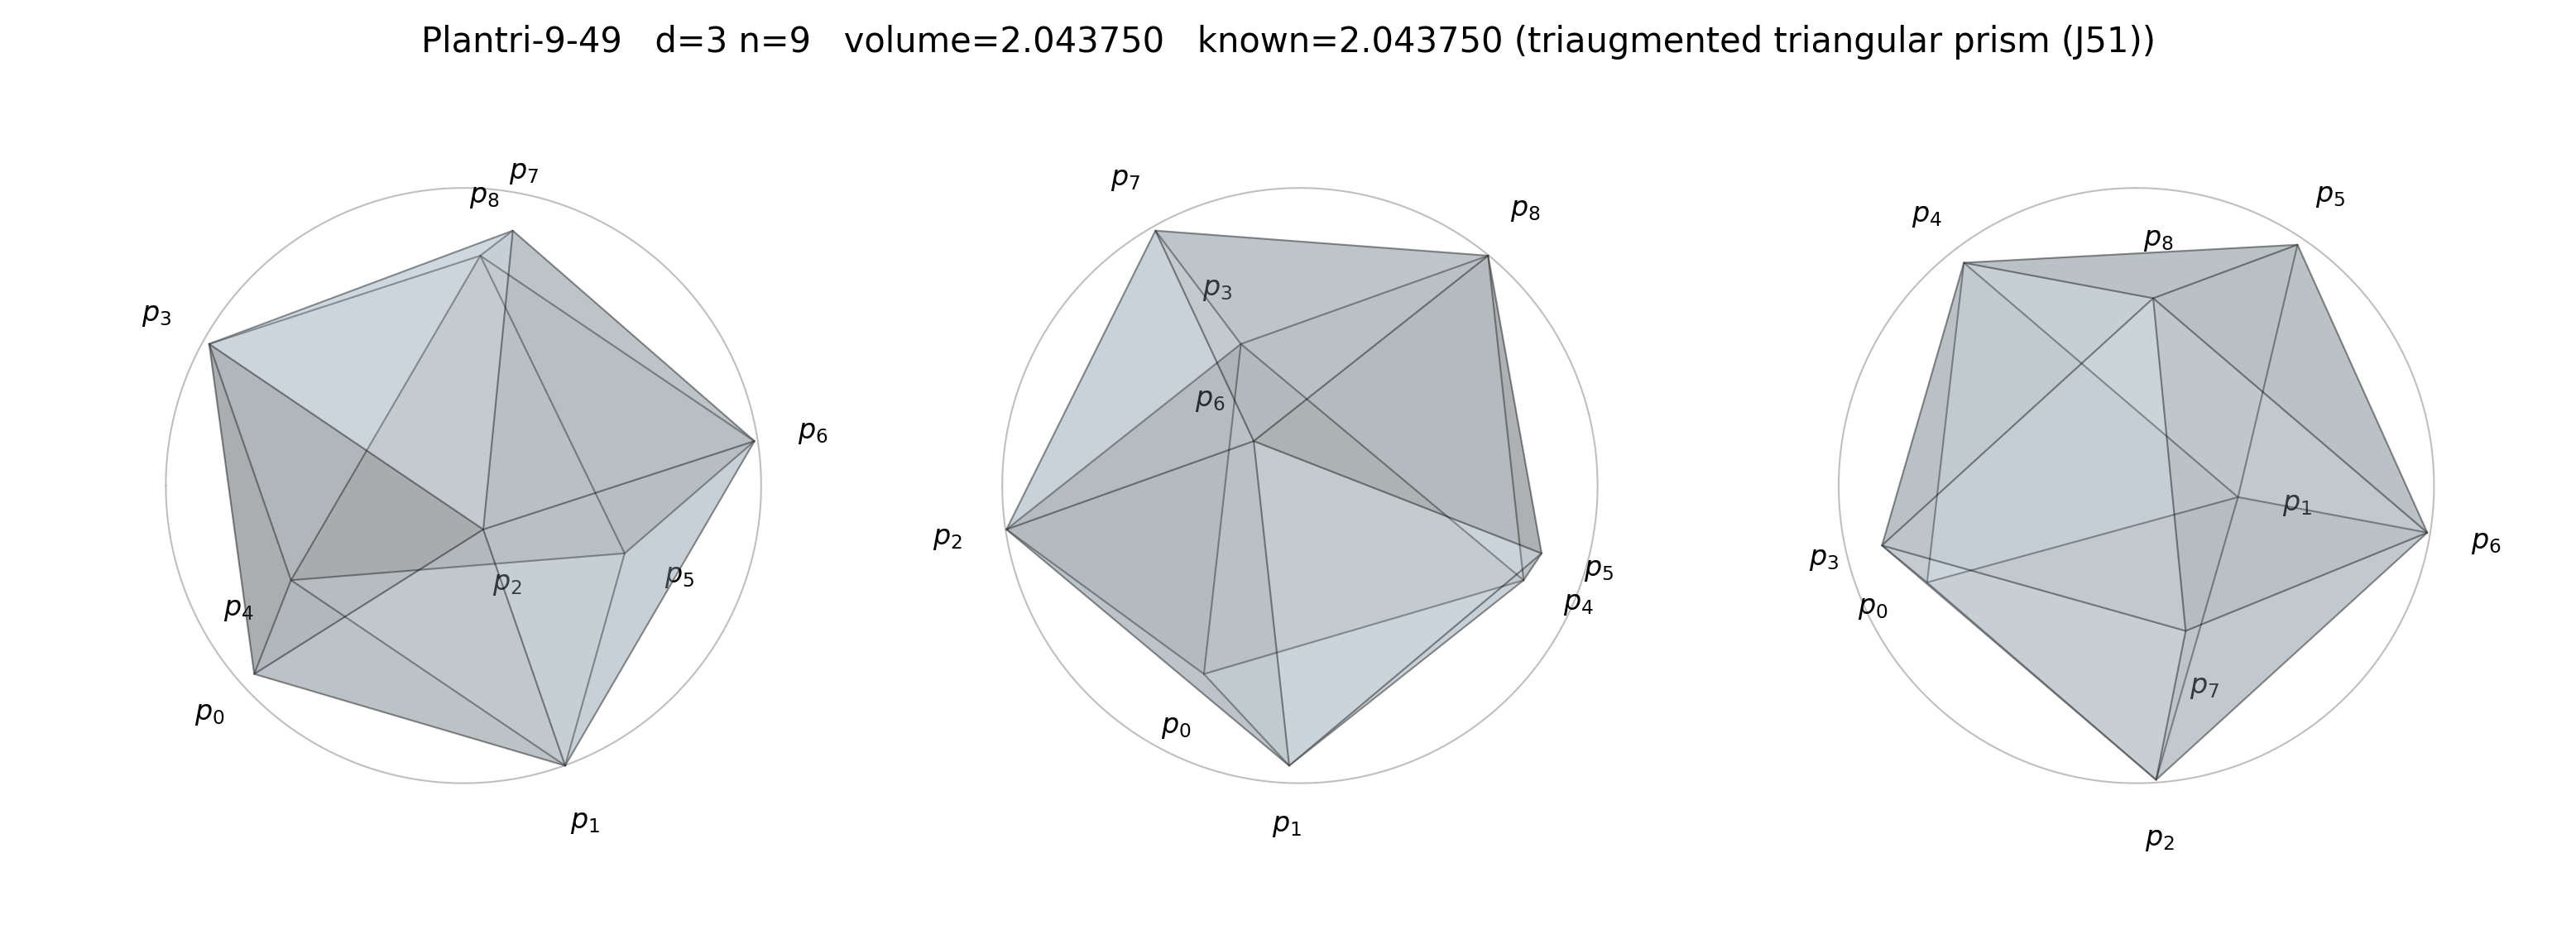
\includegraphics[width=\textwidth]{d3-n09.png}
  \caption{The $n = 9$ maximiser, three views. Vertices $p_{0},\dots,p_{8}$ on
    $\mathbb{S}^{2}$; the type is \texttt{plantri-9-49}, the triaugmented
    triangular prism.}
  \label{fig:d3n09}
\end{figure}

\subsection{Triage}

The relaxation triage of Section~\ref{sec:triage} behaves very differently
across this range \artref{cases}. Writing rivals for the non-winning types of a
case:

\begin{center}
\begin{tabular}{lrrrrrrrrr}
  \toprule
  $n$ & 4 & 5 & 6 & 7 & 8 & 9 & 10 & 11 & 12 \\
  \midrule
  rivals & 0 & 0 & 1 & 4 & 13 & 49 & 232 & 1248 & 7594 \\
  hard   & 0 & 0 & 0 & 0 & 0  & 3  & 40  & 584  & 5375 \\
  level  & E1 & E1 & E3 & E3 & E3 & E1 & E1 & E1 & E1 \\
  \bottomrule
\end{tabular}
\end{center}

At $n = 6, 7, 8$ every rival is excludable, so these cases reach E3. At $n = 4$
and $n = 5$ the enumeration holds a single type, so there is no rival to
exclude and the case stays at E1 however complete it is. From $n = 9$ onwards
the hard set is non-empty and E3 is unavailable; the heptagonal bipyramid of
Section~\ref{sec:trap} is one of the three hard types there. By $n = 11$ the
relaxation fails to separate $584$ of $1248$ rivals.

The $n = 12$ sweep covers all $7595$ types, including those with a degree-3
vertex, and returns the icosahedron \artref{cases}. Its $31$ feasible types
include $9$ with a degree-3 vertex, the largest of them at $2.370904$, so
restricting to minimum degree $4$ would have discarded inscribed polytopes and
not folds alone \artref{testtables}.

\section{Results in four dimensions}
\label{sec:results4}

\subsection{Exhaustive sweeps}

Horv\'{a}th and L\'{a}ngi extended Property Z to all dimensions, proved that
maximisers are simplicial, and solved $n = d+2$, together with $n = d+3$ for
odd $d$ and among noncyclic polytopes for even $d$; they also proved that the
maximal-volume cross-polytope inscribed in $\mathbb{S}^{d-1}$ is the regular
one \cite{horvath-langi-2016}. Because a maximiser is simplicial and
Firsching's enumeration is complete for $n \leq 8$, a per-type sweep addresses
numerically the cross-class question those results leave open \artref{cases}.

\begin{center}
\begin{tabular}{lrrrr}
  \toprule
  $n$ & 5 & 6 & 7 & 8 \\
  \midrule
  types  & 1 & 2 & 5 & 37 \\
  winner & $25\sqrt{5}/384$ & $9/32$ & $\sqrt{3}/4$ & $2/3$ \\
  level  & E1 & E3 & E3 & E3 \\
  \bottomrule
\end{tabular}
\end{center}

At $n = 5$ the enumeration holds a single type, so as at $d = 3$, $n = 4, 5$
there is no rival to exclude and the case stays at E1. Two of the others
deserve comment.

At $n = 7$ the winner over all five types is $\sqrt{3}/4 = 0.433012701892$, a
triangle and a square in orthogonal planes. The cyclic type $C_{4}(7)$, degree
sequence $[6]^{7}$, maximises at $0.389054556345$, agreeing with the
Horv\'{a}th--L\'{a}ngi closed form $(49/192)(\cos(\pi/7) + \cos(2\pi/7))$ to
$6 \times 10^{-17}$. Because this is the maximum found over the whole cyclic
type rather than the value at one configuration, it is direct numerical
evidence for their Problem 1, that the maximal-volume cyclic polytopes in
$\mathcal{P}_{d}(d+3)$ are the congruent copies of $C_{d}(d+3)$, and for their
Problem 2, that for even $d$ the overall maximiser is not cyclic.

At $n = 8$ all $37$ types are swept and the regular cross-polytope wins at
$2/3$, ahead of the best rival in convex position, $0.533173$
(\texttt{firsching-8-5}), by $20.0\%$ of its own value. The triage strengthens
this: every rival's \emph{signed} maximum also falls below $2/3$, the largest
being $0.601260$ (\texttt{firsching-8-22}) with a $9.81\%$ margin, so the case
reaches E3. Horv\'{a}th and L\'{a}ngi prove optimality here only within the
cross-polytope class, whereas the sweep ranges over every combinatorial type,
so it covers a wider class of polytopes, though only numerically.

\subsection{The orthogonal polygon-pair family}

The winners at $n = 6, 7, 8$ share one description: $n = 6$ is two triangles,
$n = 7$ a triangle and a square, and $n = 8$ two squares, the $16$-cell, each
pair lying in orthogonal $2$-planes. Since the polygons lie in complementary
orthogonal subspaces through the origin their hull is a free sum, so with
$\operatorname{area}(P_{m}) = (m/2)\sin(2\pi/m)$,
\begin{equation}
  \label{eq:polygonpair}
  \vol_{4}(m,k)
  = \frac{2!\,2!}{4!}\operatorname{area}(P_{m})\operatorname{area}(P_{k})
  = \frac{mk}{24}\sin\frac{2\pi}{m}\sin\frac{2\pi}{k},
  \qquad m + k = n .
\end{equation}
This requires $m, k \geq 3$: a $2$-gon is a segment and spans one dimension
rather than two, which is why $n = 5$ falls outside the family and is the
regular simplex instead.

\begin{table}[ht]
  \caption{The polygon-pair family. ``Status'' records the published status;
    \emph{class-proven} means optimality was proved only inside a restricted
    class, noncyclic types at $n = 7$ and cross-polytopes at $n = 8$.}
  \label{tab:pair}
  \begin{tabular}{rlllr}
    \toprule
    $n$ & split & exact volume & numeric & status \\
    \midrule
    6  & $(3,3)$ & $9/32$ & 0.281250000000 & proven \\
    7  & $(3,4)$ & $\sqrt{3}/4$ & 0.433012701892 & class-proven \\
    8  & $(4,4)$ & $2/3$ & 0.666666666667 & class-proven \\
    \bottomrule
  \end{tabular}
\end{table}

Each row of Table~\ref{tab:pair} is the best split of its $n$ and equals the
sweep winner above. Free search \artref{free} matches every row to $10^{-15}$,
and each value is verified against the explicitly constructed polytope
\artref{families} \artref{testtables}.

The family does not stay optimal. The type-free search \artref{free} matches
the best split at $n = 9$ and $n = 10$ to $10^{-15}$, but at $n = 11, 12, 13$
it finds inscribed polytopes with all $n$ points as vertices whose volumes
$1.046529$, $1.171382$ and $1.303558$ exceed the best split by $1.65\%$,
$4.12\%$ and $10.01\%$ \artref{testtables}. Each is an explicit configuration,
so the family is not optimal for these $n$; at $n = 9, 10$, where the
enumeration of types is no longer complete, its optimality is neither shown nor
refuted.

\section*{AI assistance}
An AI assistant was used as an exploratory tool during the development of the
method presented here, including for mathematical discussion, implementation,
and the exploration of alternative approaches. The underlying idea is the
author's, and the method was evaluated by the author against existing
mathematical results.
\section*{Code and data}
\label{sec:artifacts}
{\footnotesize
Everything reported here is available at \repohref. The entries below are cited
as [R$k$]; they are artifacts rather than literature and are numbered separately
from the bibliography. Case and free-search records follow the pattern
\texttt{d3-n19.json}, with the dimension and vertex count encoded in the
filename, so a claim about a particular $(d, n)$ resolves to a single file.
\begin{artifactlist}
\artifact{reproduce}{scripts/reproduce.py}{reruns the sweeps against their
recorded values, exiting nonzero on any drift}
\artifact{cases}{results}{the case records, one per swept $(d, n)$}
\artifact{evidence}{src/inscribed/store/case.py}{the evidence levels,
recomputed from the per-type records on load; tests in
\artpath{tests/test_store.py}}
\artifact{plantri}{src/inscribed/enumeration/plantri.py}{the $d = 3$ type
source, wrapping \texttt{plantri}; counts in
\artpath{tests/test_enumeration.py}}
\artifact{firsching}{src/inscribed/enumeration/firsching.py}{the $d = 4$ type
source, reading Firsching's inscribed realisations; counts in
\artpath{tests/test_enumeration.py}}
\artifact{ascent}{src/inscribed/search/ascent.py}{the exact vertex step and
Algorithm~\ref{alg:ascent}; monotonicity in
\artpath{tests/test_search.py}}
\artifact{maximize}{src/inscribed/search/maximize.py}{multistart maximisation
within one type; seeding in \artpath{tests/test_search.py}}
\artifact{sweep}{src/inscribed/search/sweep.py}{the two-pass sweep over a type
list; tests in \artpath{tests/test_sweep.py}}
\artifact{validation}{src/inscribed/analysis/validation.py}{the
convex-position certificate and the Property~Z check; tests in
\artpath{tests/test_validation.py}}
\artifact{symmetry}{src/inscribed/analysis/symmetry.py}{symmetry groups read
off the quantised Gram matrix; group orders in
\artpath{tests/test_symmetry.py}}
\artifact{free}{results/free}{the type-free search records of
Section~\ref{sec:results4}; tests in \artpath{tests/test_fourd.py}}
\artifact{catalog}{src/inscribed/catalog/data.py}{the published values, closed
forms and statuses quoted in the tables}
\artifact{families}{src/inscribed/catalog/families.py}{the closed-form
families, including the orthogonal polygon pair; each checked against its
own construction in \artpath{tests/test_families.py}}
\artifact{testtrap}{tests/test_star_bipyramid.py}{tests backing
Section~\ref{sec:trap}}
\artifact{testmethod}{tests/test_paper_method.py}{tests backing the counts
and tolerances of Section~\ref{sec:method}}
\artifact{testtables}{tests/test_paper_tables.py}{tests backing the tables
and quoted figures of Sections~\ref{sec:results3} and \ref{sec:results4}}
\artifact{testcatalog}{tests/test_families.py}{tests backing the catalog
against its cited sources}
\end{artifactlist}
}
\bibliographystyle{amsplain}
\bibliography{references}
\end{document}